In this lab we will be installing virtual machines for the Kali Linux, Oracle Linux, Windows 10, and optionally Windows Server 2012 R2 operating systems.
Originally I had decided to install these using Windows Hyper-V but I was having issues with the network configurations so I switched to Oracle's VirtualBox VM Manager.

\begin{figure}[H]
    \centering
    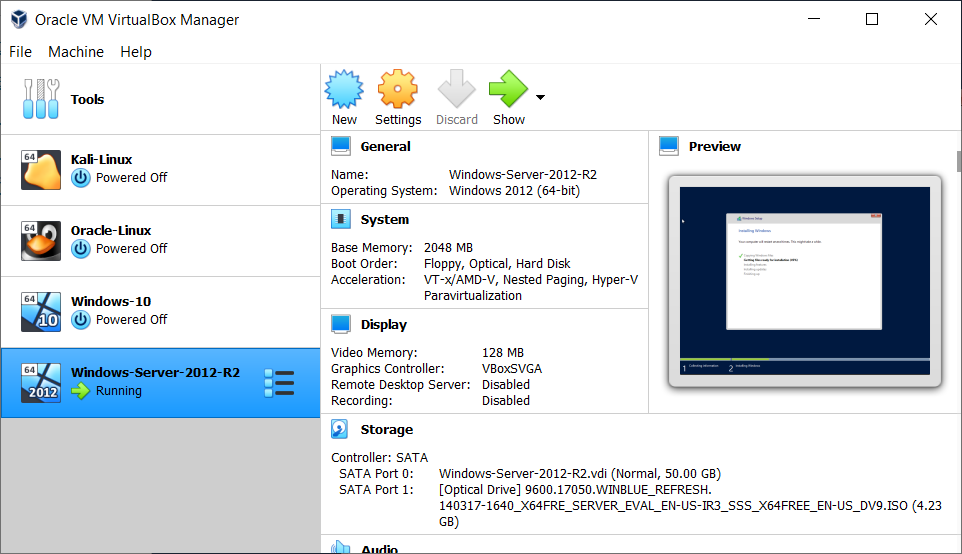
\includegraphics[width=\linewidth]{figures/Virtualbox-Home.png}
    \caption{Home screen of VirtualBox software.}
\end{figure}
This screenshot shows the overview of what VMs are installed and allows access to the settings for each.

\begin{figure}[H]
    \centering
    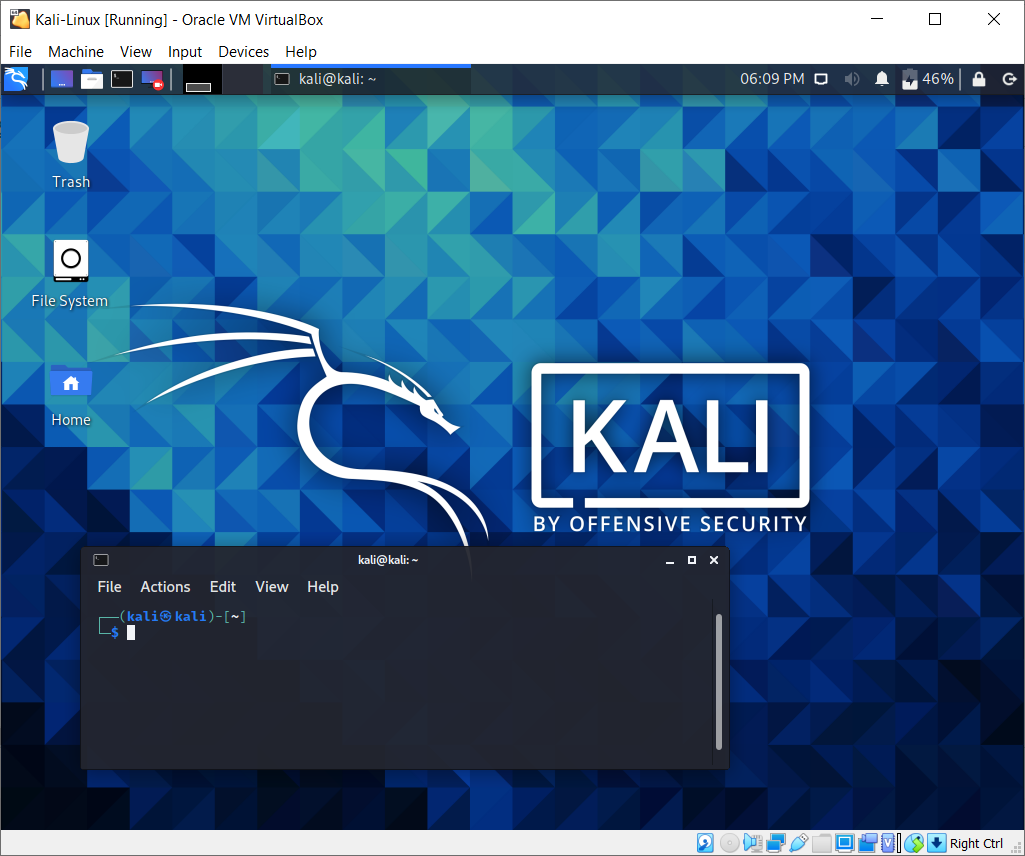
\includegraphics[width=\linewidth]{figures/Kali-Home.png}
    \caption{Kali linux desktop and terminal.}
\end{figure}
Here is proof that Kali linux is installed and operable as a virtual machine.

\begin{figure}[H]
    \centering
    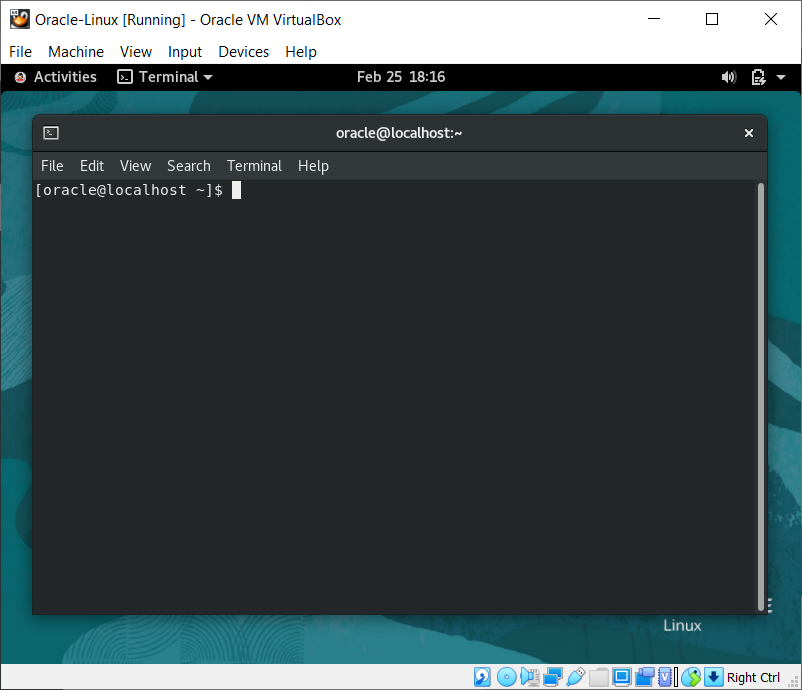
\includegraphics[width=\linewidth]{figures/Oracle-Home.png}
    \caption{Oracle linux desktop}
\end{figure}
This is the desktop of Oracle linux showing that it is installed as a VM.

\begin{figure}[H]
    \centering
    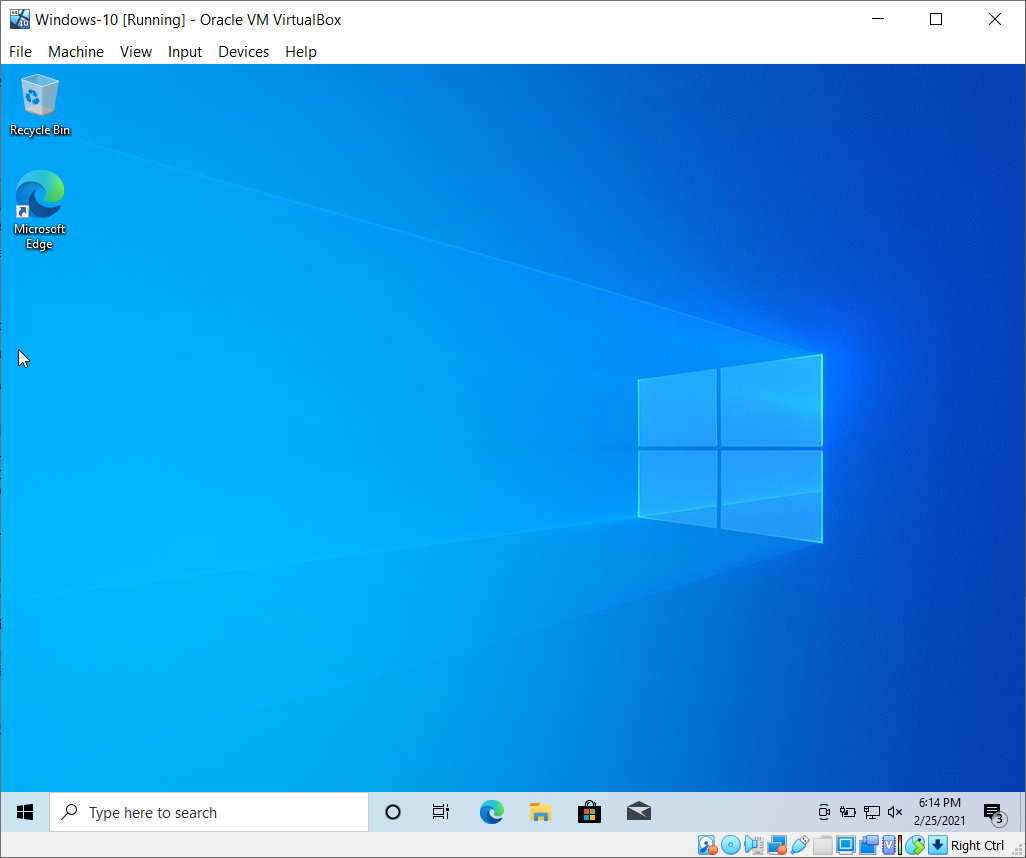
\includegraphics[width=\linewidth]{figures/Windows-10-Home.png}
    \caption{Windows 10 desktop.}
\end{figure}
This shows that Windows 10 is installed as a VM.
In order for me to be able to login I had to create a new Outlook email similar to my school email.

\begin{figure}[H]
    \centering
    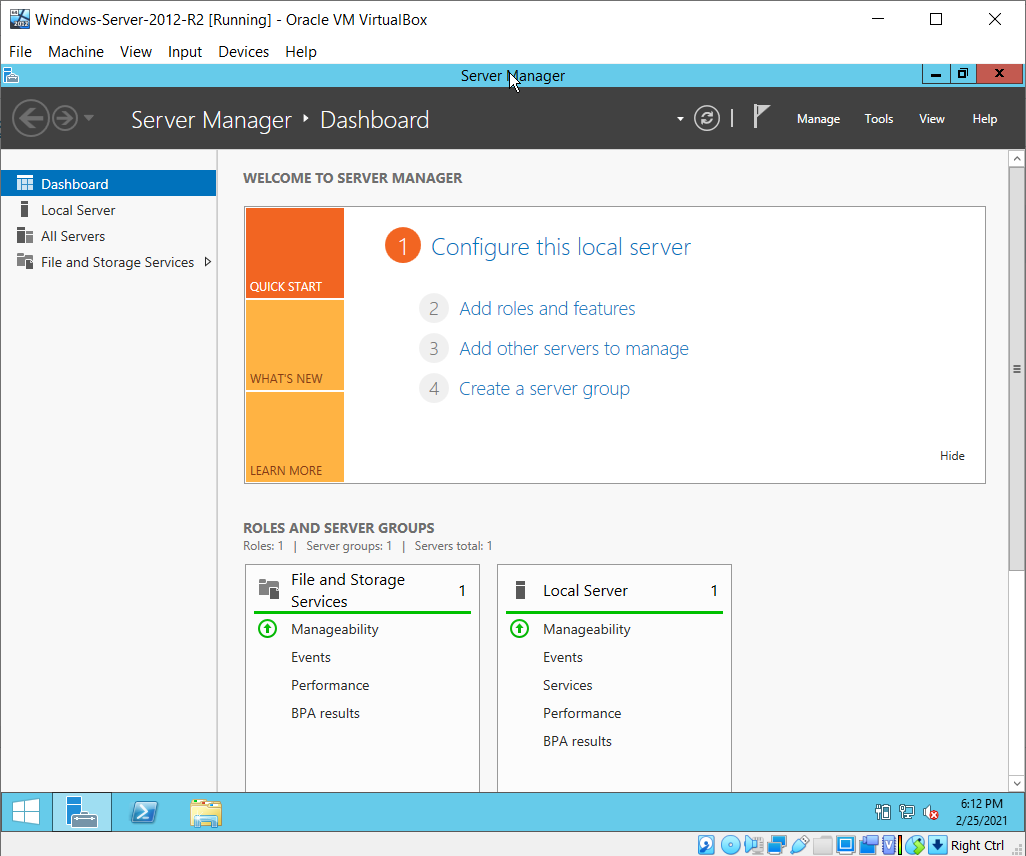
\includegraphics[width=\linewidth]{figures/Windows-2012-Home.png}
\end{figure}
This is the Windows Server 2012 R2 server manager screen that shows when starting the virtual machine.

In this lab we learned how to install virtual machines.
Every virtual machine has a different setup process because of the different operating systems and uses of the VM.
Originally I had planned to install all of these via Windows Hyper-V because I have that on my system, however I had complications with setting up the virtual switch configuration.
So I had to migrate to VirtualBox to complete the assignment.
During this process I learned a lot about how Hyper-V handles virtual networks via switch configurations and bridged networks.
VirtualBox's network setup is easier out of the box so I did not have any of the issues with VirtualBox that I was having with Hyper-V.